\subsection{RENEW ROI CRITERIA}
%Diagrama2
The $ROI$ is an important element in the algorithm, because of that this  
will be used as pattern to find a match of tracked object at the current image. 
The  question in this case is to know the best moment to refresh the $ROI$
with a new perspective of object. 
Here, we establish the criteria that when the comparison of images return 
a $PCC$ lower than $0.925$ and greater than $0.8$, then the $ROI$ is changed with the current 
analyzed region and a new position of $ROI$ is establish with $(x_i,y_i,d_i)$. 
Thus, it was adopted as $0.8$ the lower limit to a match case\cite{Eugene},
see Fig. \ref{fig:newroicri}. Values less than $0.8$ cause a  lost object alert.
Finally, it is important to note that if the $ROI$ is changed, the new $ROI$ is establish
with the real size of the analyzed region and not with the rescaled version used
in the calculus of the $PCC$.


\begin{figure}[H]
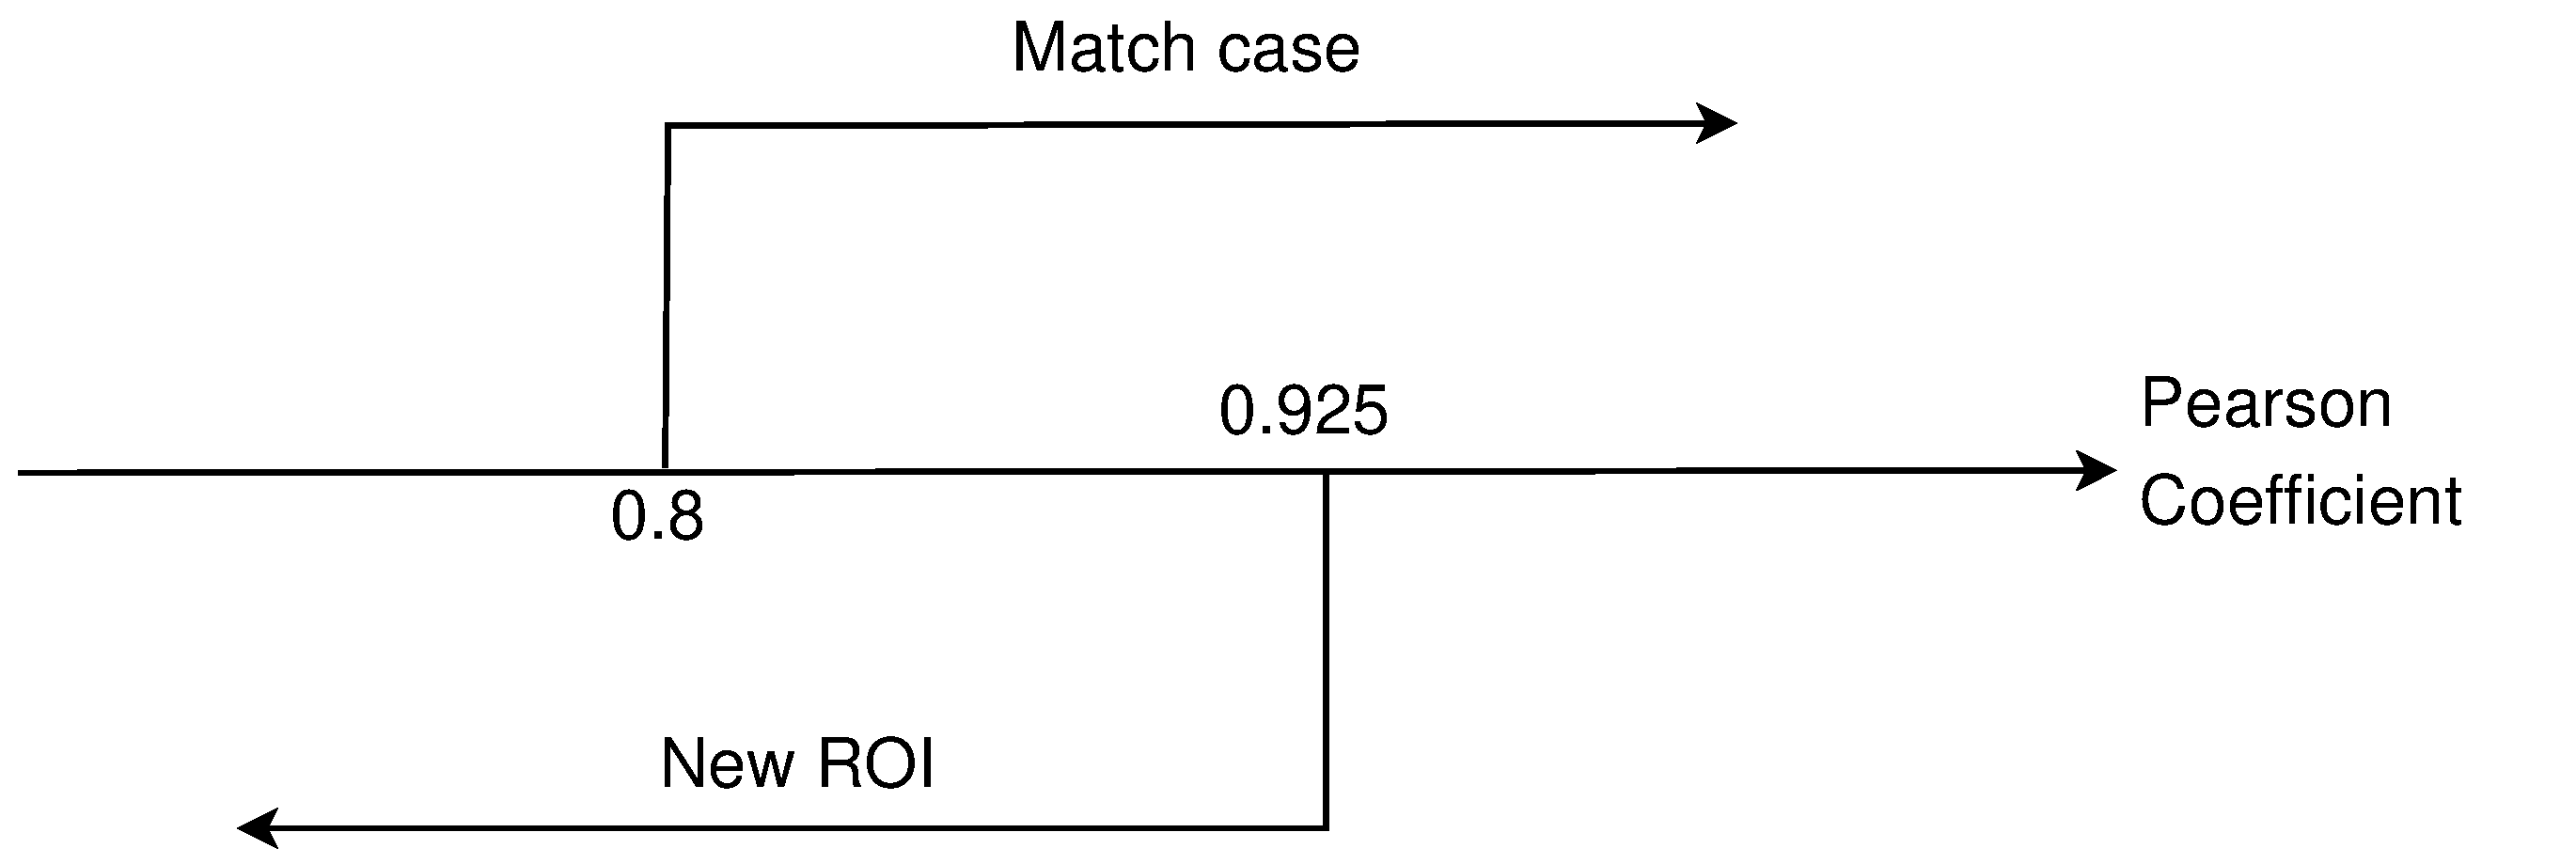
\includegraphics[width=\columnwidth]{images/figure3.eps}
\caption{When the comparison is greater than $0.8$, including numbers bigger than 
$0.925$, means that the target was matched. But if two regions are compared 
and the $PCC$ is less than $0.925$ and greater than $0.8$, 
then the $ROI$ changes to the current analyzed region.}
\label{fig:newroicri}
\end{figure}

The system needs to have high level of reliability, so that the lower limit adopted 
contributes to an operation with minimum of mistakes.
